\subsection{Approach to Fix \approachName's Preference Bias}
In the previous section, we discovered that MongoDB's \approachName optimizer misses collection scans that are superior to the chosen plan. 
 Therefore we made an improvement that lets MongoDB consider collection scans.
We suppose this might just be a bug in the program, and we 
expected the problem can be solved after we add COLLSCAN to 
the candidates. Therefore, we modify the MongoDB source code
to let it consider the collection scan as a candidate query plan. 
After the simple fix we confirm that the modified version of MongoDB successfully
examines COLLSCAN for all cases. For example, we repeat the case
in which all documents are retrieve, and Figure~\ref{fig:qexp2}
illustrates that our modified MongoDB successfully examines COLLSCAN 
as a candidate. 

We repeat the experiment on MongoDB V2 after verifying the 
change we made is effective. Nevertheless, we obtain the 
same visualization results as V1. In contrast to our expectation, 
we notice that all collection scans are rejected during the 
experiment. 

The results we observed confirm that the problem is not just 
a bug in the MongoDB 4.4.0 source code; the problem is 
related to the underlying query planning mechanism of MongoDB, 
the \approachName approach. We have come to the conclusion that there 
is a major weakness in the current implementation of \approachName. The
experiment results demonstrate that the current \approachName approach
has a preference bias. As a result, the query optimizer might 
stick on index scans while collection scans are theoretically 
a better choice.

% \begin{figure}[h]
%     \centering
%     \includegraphics[width=\linewidth]{images/rest1/rejected.png}
%     \caption{Query explain of the 100\% selective query: after a simple fix}
%     \label{fig:qexp2}
% \end{figure}

\subsection{Exploring the impact of the preference bias issue}
In this section, we present a new experiment design which
is capable of quantifying and visualizing the impact of the 
preference bias issue. To begin with, we use an empirical 
method to compare the query plan choices of MongoDB V2 with
the real best options to measure the degree of defects for
the current implementation of \approachName. As the previous design 
only focuses on the uniformly distributed data set, we 
enrich the physical design by considering both symmetric 
(skew) and asymmetric (no skew) database design. Moreover, 
we examine the physical design where only one index is
available in the database. We observe that the skewness of
the dataset does not influence MongoDB's query plan decision.

\subsubsection{Database Physical Design}
In this experiment, we test against MongoDB V2. We populate
one database with four collections, each collection contains
$1 \times 10^5$ documents. Similar to the experiment in Part 2,
each document has two integral fields, namely A and B. A 
positive integer in the range $(0, 1\times 10^5]$ is assigned
to each field.

However, we run experiments on both skewed (symmetric) and 
asymmetric (no skew) data set. More specifically, values 
assigned to field B have different kinds of distributions,
while values of field A remains uniform distribution, as 
shown in table \ref{table:data-dist}. Case 1 is exactly the same 
case we used in the previous experiment.
In Case 2 to 4 we generate various kinds of data distribution 
via discrete random number generator of \verb|scipy| and 
\verb|numpy| packages. Figure \ref{fig:case1}, \ref{fig:case2}, 
\ref{fig:case3} and \ref{fig:case4} illustrates the data 
distribution the dataset that we will cover. In case 5 to 
8 we drop the index on A to explore the behavior of MongoDB V2.

\begin{table}[h]
\begin{tabular}{lllll}
    \toprule
    Case Number & Distribution of A & Distribution of B & Index on A & Index on B \\ 
    \midrule
    1           & Uniform           & Uniform           & True       & True       \\
    2           & Uniform           & Linear            & True       & True       \\
    3           & Uniform           & Normal            & True       & True       \\
    4           & Uniform           & Zipfian           & True       & True       \\
    5           & Uniform           & Uniform           & False      & True       \\
    6           & Uniform           & Linear            & False      & True       \\
    7           & Uniform           & Normal            & False      & True       \\
    8           & Uniform           & Zipfian           & False      & True      \\
    \bottomrule
    \end{tabular}
    \caption{Data distribution of field A and field B}
    \label{table:data-dist}
\end{table}

\begin{figure}[h]
    \subfigure{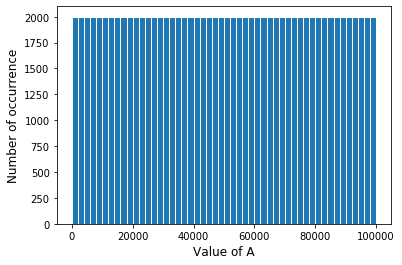
\includegraphics[width=0.4\linewidth]{images/body/uniforma.png}} 
    \subfigure{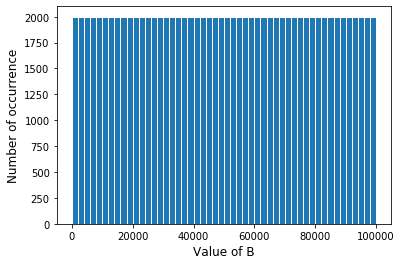
\includegraphics[width=0.4\linewidth]{images/body/uniformb.png}} 
    \caption{Case 1 \& 5 data distribution}
    \label{fig:case1}
\end{figure}

\begin{figure}[h]
    \subfigure{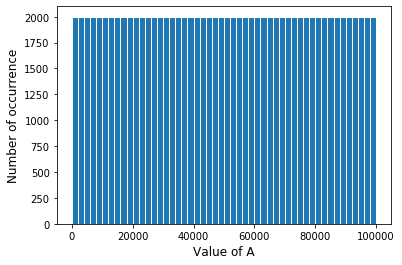
\includegraphics[width=0.4\linewidth]{images/body/uniforma.png}} 
    \subfigure{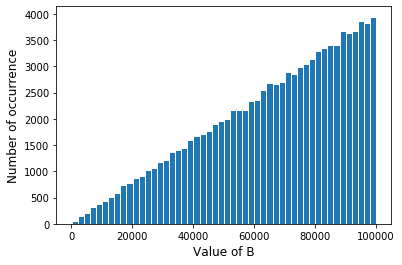
\includegraphics[width=0.4\linewidth]{images/body/linear.png}} 
    \caption{Case 2 \& 6 data distribution}
    \label{fig:case2}
\end{figure}

\begin{figure}[h]
    \subfigure{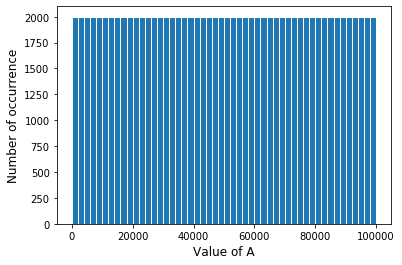
\includegraphics[width=0.4\linewidth]{images/body/uniforma.png}} 
    \subfigure{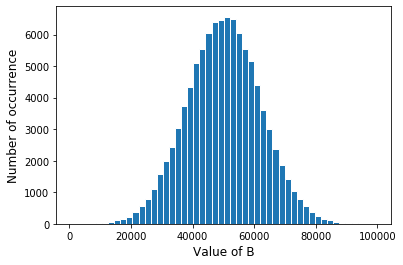
\includegraphics[width=0.4\linewidth]{images/body/normal.png}} 
    \caption{Case 3 \& 7 data distribution}
    \label{fig:case3}
\end{figure}

\begin{figure}[h]
    \subfigure{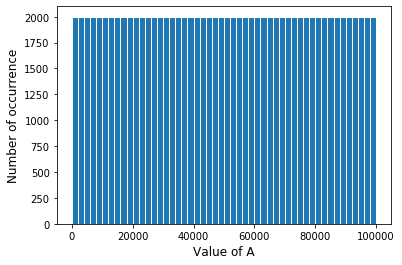
\includegraphics[width=0.4\linewidth]{images/body/uniforma.png}}
    \subfigure{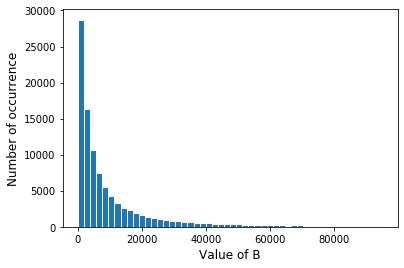
\includegraphics[width=0.4\linewidth]{images/body/zipf.png}} 
    \caption{Case 4 \& 8 data distribution}
    \label{fig:case4}
\end{figure}


\subsubsection{Quantify The Impact}
Given that MongoDB V2 prefers the index scan more than 
collection scans, we aims to explore the impact of this
issue. We adopt an empirical method to quantify the 
impact. We designed a impact factor $\delta$ which 
indicates how worse the query plan is in comparison 
with the ideal baseline. We obtain the ideal baseline
through a group of experiments. 

The ideal baseline is directly related with the execution
time of the real best query plan among all candidate plans.
That is to say, the execution time of a query should be 
the shortest with a real best query plan; it is impossible
to further improve the query performance through switching
other query execution strategies. The query execution time,
our vital metric, can be obtained by inspecting query
execution statistics. During the experiment, we extract the \verb|executionStats.executionTimeMillis| field to retrieve
the wall-clock time in milliseconds required for the query 
plan evaluation and query execution.

If there are multiple query plan candidates, we determine
the real best candidate by measuring and comparing the 
execution time of each query plan candidate. As we mentioned
in the section \ref{sec:hint}, MongoDB provides users 
a \verb|hint(<queryPlan>)| method to customize execution 
plan. We use this method to force the query optimizer to 
execute each candidate plan. After executing all query plans,
the one with the shortest execution time is the real best 
query plan. We use the visualization technique explained in 
the section \ref{sec:vm} to visualize all real best plans in 
the 2D coordinate. Similar to the experiment in Part 2, we 
find the real best query plan through a majority vote. We 
repeat this experiment ten times to measure the mean execution
time of the real best query plan. 

In addition, we visualize the impact of the defect using 
a heatmap. The color of the pixel (i,j) in the heatmap is 
determine by the value of $\delta_{i,j}$. After recording
the execution time of all real best query plans. We use 
the same technique to obtain the execution time of query 
plans selected by MongoDB V2. And then we can calculate 
the value of $\delta_{i,j}$ using the mean execution time 
of the query plans selected by MongoDB V2 and that of the
real best query plans:

\begin{equation}
    \delta_{i,j} = \frac{\sum\limits_{n=1}^{N}t_{i,j,n}}{\sum\limits_{n=1}^{N}t_{i,j,n}^{'}}
\end{equation}

\begin{equation}
    \delta_{i,j} = \frac{\sum\limits_{n=1}^{N}t_{i,j,n}}{\sum\limits_{n=1}^{N}t_{i,j,n}^{'}}
\end{equation}

\begin{equation}
    \delta = \frac{t_{chosen}}{t_{optimal}}
\end{equation}

, where N is the number of repetition, $t_{i,j,n}^{'}$ 
is the execution time of the query plan at (i,j) selected
by MongoDB V2 in the $nth$ repetition, and $t_{i,j,n}$ is
the execution time of the real best query plan at (i,j) 
in the $nth$ repetition. 

For each visualization, we express the overall performance
difference ($\Delta_p$) between the ideal query plans and
the actual ones in terms of mean query execution time. For
the $(ith, jth)$ query, we denote the mean execution time 
of its optimal query plan as $\mu_{i,j}$ and that of the 
actual query plan as $\mu_{i,j}^{'}$.

\begin{equation}
    \Delta_p = \frac{\sum\limits_{j=0}^{D-1}(\sum\limits_{i=0}^{D-1}\mu_{i,j}^{'}) - \sum\limits_{j=0}^{D-1}(\sum\limits_{i=0}^{D-1}\mu_{i,j})}       {\sum\limits_{j=0}^{D-1}(\sum\limits_{i=0}^{D-1}\mu_{i,j})}
\end{equation}

\begin{equation}
    \Delta_p = \frac{\sum\limits_{j=0}^{D-1}(\sum\limits_{i=0}^{D-1}t_{i,j}^{'}) - \sum\limits_{j=0}^{D-1}(\sum\limits_{i=0}^{D-1}t_{i,j})}       {\sum\limits_{j=0}^{D-1}(\sum\limits_{i=0}^{D-1}t_{i,j})}
\end{equation}

$D$ is the dimension of the grid. A negative value of 
($\Delta_p$) indicates the performance is worse than the 
optimal case.

The accuracy of the query optimizer can be calculated as:
\begin{equation}
    accuracy = \frac{\text{correctly predicted cases}}{\text{total number of cases}} \times 100\%
\end{equation}

\subsubsection{Handling Outliers}
When we gather execution times of all query plans, we note
that there are less than ten outliers which deviate markedly 
from other data points. These outliers are usually fifty 
times higher than the mean value. We suppose that the 
unstable performance of T2.micro instance is very likely 
to be the cause. Therefore, we identify those outliers, 
and drop them using 1.5 IQR (interquartile range) rule. 
We measure the interquartile range for $t_{i,j,1}^{'}, 
t_{i,j,2}^{'}, ..., t_{i,j,N}^{'}$ and then multiply the
interquartile range (IQR) by the factor 1.5. Any data point
greater than the sum of the third quartile and 1.5 IQR is 
droped; any number less than the difference of the first 
quartile and 1.5 IQR is dropped as well.


\subsection{Unfair "Race"}
As we mentioned in Section~\ref{sec:fptp}, the \approachName approach execute all query plans in RR fashion and the first candidate returns the initial batch of results (i.e. 101 matched documents) is chosen as the execution plan. However, in the practices we found that the documents "allowed" to be examined by collection scans is always one unit less than index scans. This implementation detail forms an unfair "races" between a collection scan and an index scan, and it makes the query optimizer prefers the index scan more than collection scan. We demonstrate this phenomenon through a boundary case study. 

\begin{table}[h]
    \begin{tabular}{lllll}
    \toprule
    Case Number & Distribution of A & Distribution of B & Index on A & Index on B \\ 
    \midrule
    1           & Uniform           & Uniform           & True       & True       \\ 
    \bottomrule
    \end{tabular}
    \caption{The database design of the boundary case}
    \label{tbl:irc}
\end{table}


The physical design of the database is identical to the one we used in Part 2. We study the most generic case, in which the distribution of field A and field B are identical, Table \ref{tbl:irc} shows the database design. We simulate the boundary case in which the selectivity of the query equals one. For instance, we use the following query in our case study:

\vspace{0.02\linewidth}
\begin{algorithm}[htbp]
\floatname{algorithm}{}
\caption{Example Query (MongoDB Query)}
\begin{verbatim}
db.collection.find({
        "A" : {"$gte" : 0, "$lt" : 100000},
        "B" : {"$gte" : 0, "$lt" : 100000}
    })
\end{verbatim}
\label{query_mongo}
\end{algorithm}


In this case, a collection scan is clearly the winner since it does not have the overhead of retrieving index documents. However, the query explain indicates that total documents can be examined by the collection scan is only 100, which is one unit less than index scan. As a result, the potential number of documents \verb|nReturned| can be returned by a collection scan can never reach 101. Therefore in such cases, a collection scan can never outperform an index scan.

\subsection{Overrated Index Scan}
The main cause of the preference bias is the current implementation of \approachName approach overrates the index scan. We demonstrate this point using another case study. This case study use the same database design and workload as the previous one, except for we modify the range predicates of the query:

\vspace{0.02\linewidth}
\begin{algorithm}[htbp]
% \renewcommand{\thealgorithm}{}
\floatname{algorithm}{}
\caption{Example Query (MongoDB Query)}
\begin{verbatim}
db.collection.find({
        "A" : {"$gte" : 0, "$lt" : 95000},
        "B" : {"$gte" : 0, "$lt" : 95000}
    })
\end{verbatim}
\label{query_mongo}
\end{algorithm}

In this case, we ensure the selectivity of both range predicates equal to 0.95. The experiment set up is identical to the case 1 in chapter \ref{chap:exp2}, therefore we can obtain the optimal query plan of this query from the visualization results shown in figure \ref{fig:linearreal}. According to the visualization, the optimal candidate is a collection scan, while the winning plan is an index scan. By inspecting the query execution log, we found that the query optimizer overrates the $productivity$ of the index scan.

We explained that the \approachName approach assign a score to summarize the performance of each query plan in the final round of evaluation. The query plan has the highest score will be chosen. The formula considers the $productivity$ of each query plan, and the way of calculating the productivity is:

\begin{equation}
    productivity = \frac{queryResults}{workUnits}
\end{equation}

When measuring the workUnit of an index scan, the \approachName approach ignores the cost of fetching index documents; it measured the index retrieving work and and the document retrieving work together as a single unit of work (i.e. the same amount of work required by a collection scan). Therefore, in practice, the $productivity$ of an index scan is overrated. This implementation detail erases the advantage of a collection scan. As the overhead of an index scan is not measured, it is very likely an index scan is measured as outperforming a collection scan in all cases.


% \subsection{Suggestions For Improvements}

% Given that MongoDB overrates the index scan. We believe that a possible suggestion for improvement is dynamically adjusting the productivity score of index scan based on the difficulty in retrieving the index document. As the implementation of \approachName relies on empirical results, we suggest MongoDB measure the work in retrieving the index document in terms of the unit of work. 

% In the previous section, we found that collection scans were given a penalty of $-1$ advance. We think this was an accident, and we can remove this penalty to solve the problem.


\subsection{Limitations}
In this work, we use simple and generic database designs to explore and evaluate MongoDB's \approachName query optimizer. We recognize that such simple workloads lack variety. For example, the documents only consist of numerical fields, and we do not examine complex queries which involve aggregations and various types of joins.
Also note, that we disabled MongoDB's query plan cache for the experiments. While this allows us to focus purely on how MongoDB evaluate query plans, it also means that we cannot assess how the query plan cache mechanism affects query plan evaluations. 

